\section{Проектирование программного средства} % (fold)
\label{sec:arch_and_mod}

\subsection{Разработка программного развертывания}
\label{sub:arch_and_mod:graphlib}

Прежде чем приступать к непосредственной реализации программного средства, необходимо определиться с архитектурой коллективной работы с приложением.
Во-первых, необходимо провести анализ необходимой аппаратной конфигурации, на которой будут работать части конечного программного средства, и описать их взаимодействие между собой. Для описания узлов и их связей будем использовать диаграмму развертывания:
\begin{figure}[ht]
\centering
  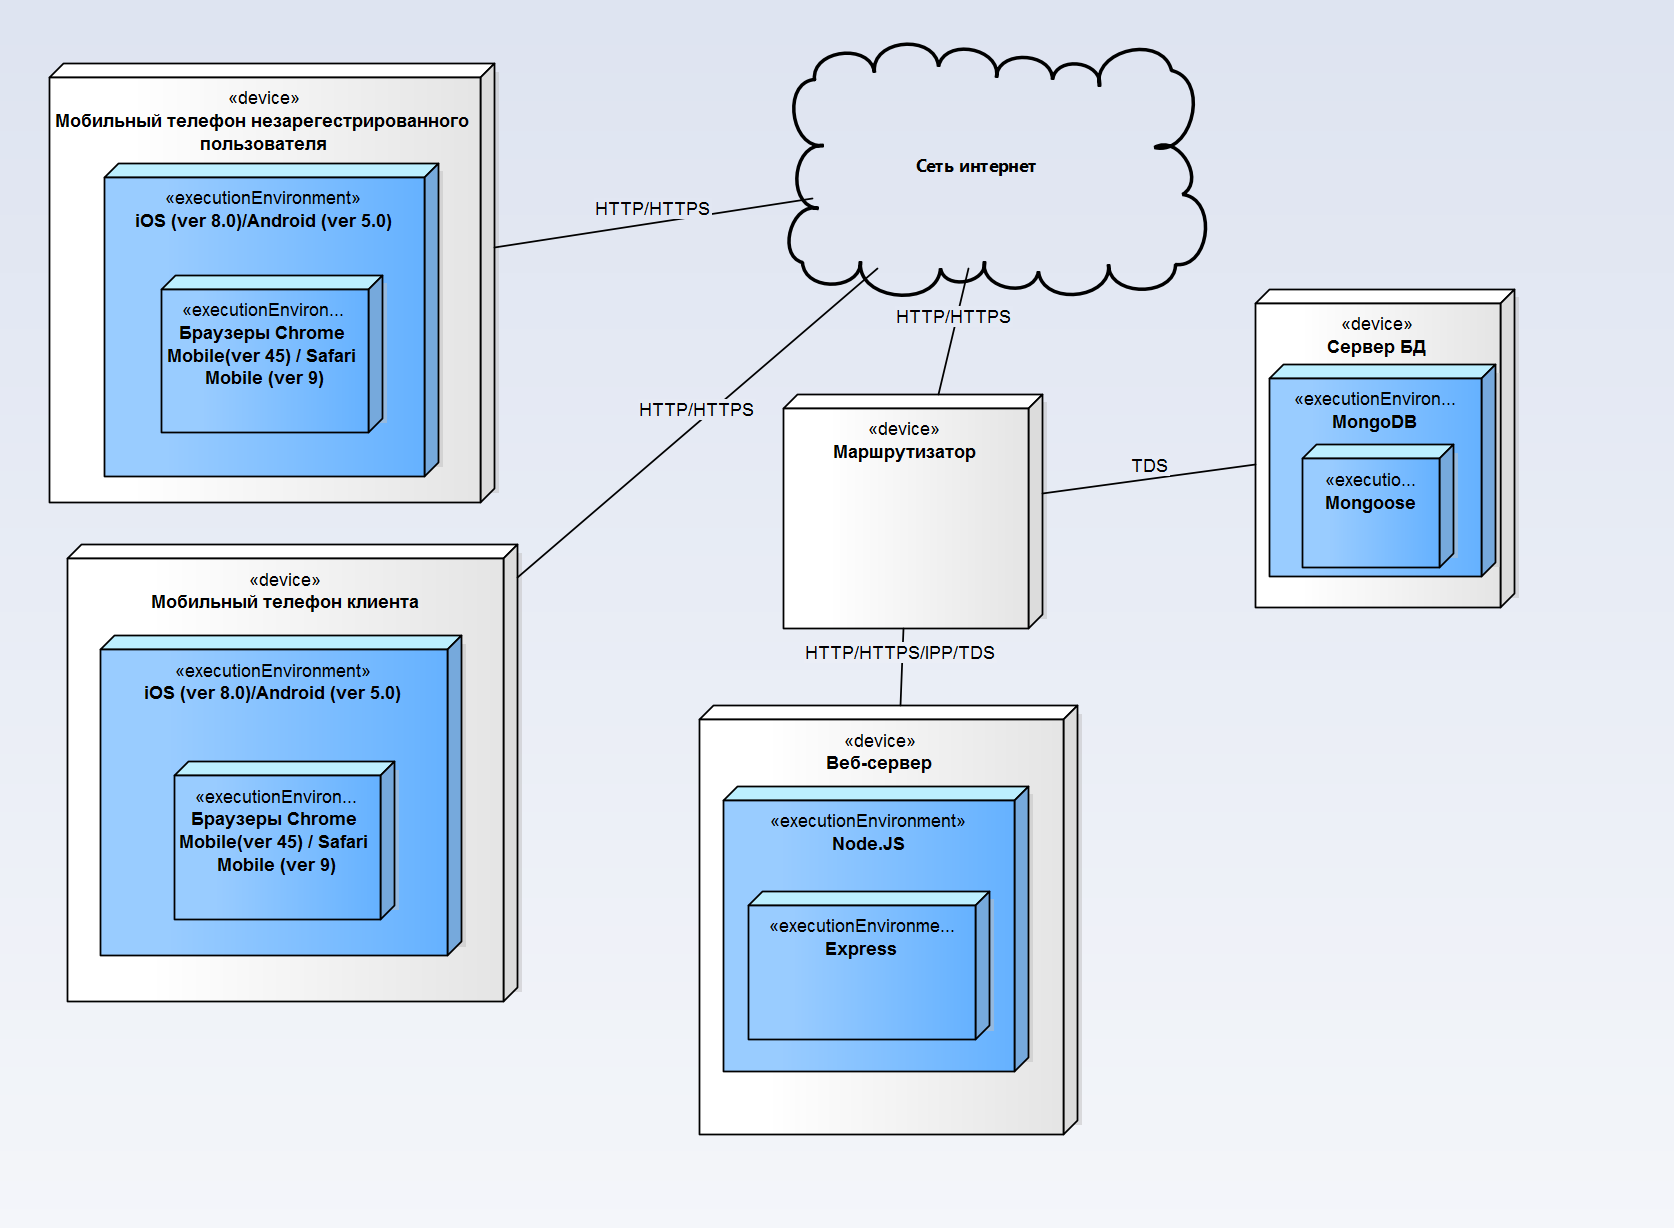
\includegraphics[scale=0.5]{device.png}  
  \caption{ Диаграмма развертывания. }
  \label{fig:domain:manual_structure:credit_device}
\end{figure}
На основе вышеизображенной диаграммы можно сделать следующие выводы:

\begin{enumerate}
  \item узлы могут располагаться в различных частях мира и взаимодействовать между собой через сеть Интернет;
  \item сервер базы данных поддерживаются в рабочем состоянии отдельно от основного сервера;
  \item клиент, осуществляющий работу с системой с помощью HTTP/HTTPS;
  \item HTTPS протокол применяется как к клиентам, так и к всевозможным серверам, с целью осуществления обмена запросами и ответами на них;
\end{enumerate}

\subsection{Разработка БД }
\label{sub:arch_and_mod:graphlib}

Перед тем, как приступать к процессу разработки, сначала нужно смоделировать базу данных, которая является оcновой будущего приложения. Чтобы база данных не вызывала трудностей при работе с ней, когда будет заполнена информацией, крайне желательно, чтобы она соответствовала трем нормальным формам:
\begin{itemize}
  \item защита от CSRF-атак (cross-site request forgery, межсайтовая подделка запроса), при которых данные пользователя могут быть переданы на другой сайт (например, сайт злоумышленника или сайт платежной системы) для совершения некой вредоносной операции;
  \item Первая нормальная форма. Переменная отношения находится в первой нормальной форме тогда и только тогда, когда в любом допустимом значении отношения каждый его кортеж содержит только одно значение для каждого из атрибутов. 
  \item Вторая нормальная форма. Переменная отношения находится во второй нормальной форме тогда и только тогда, когда она находится в первой нормальной форме, и каждый неключевой атрибут функционально полно зависит от ее потенциального ключа.
  \item Третья нормальная форма. Переменная отношения находится в третьей нормальной форме тогда и только тогда, когда она находится во второй нормальной форме, и отсутствуют транзитивные функциональные зависимости неключевых атрибутов от ключевых.
\end{itemize}

Схема базы данных разрабатываемого приложения имеет следующий вид:
\begin{figure}[ht]
\centering
  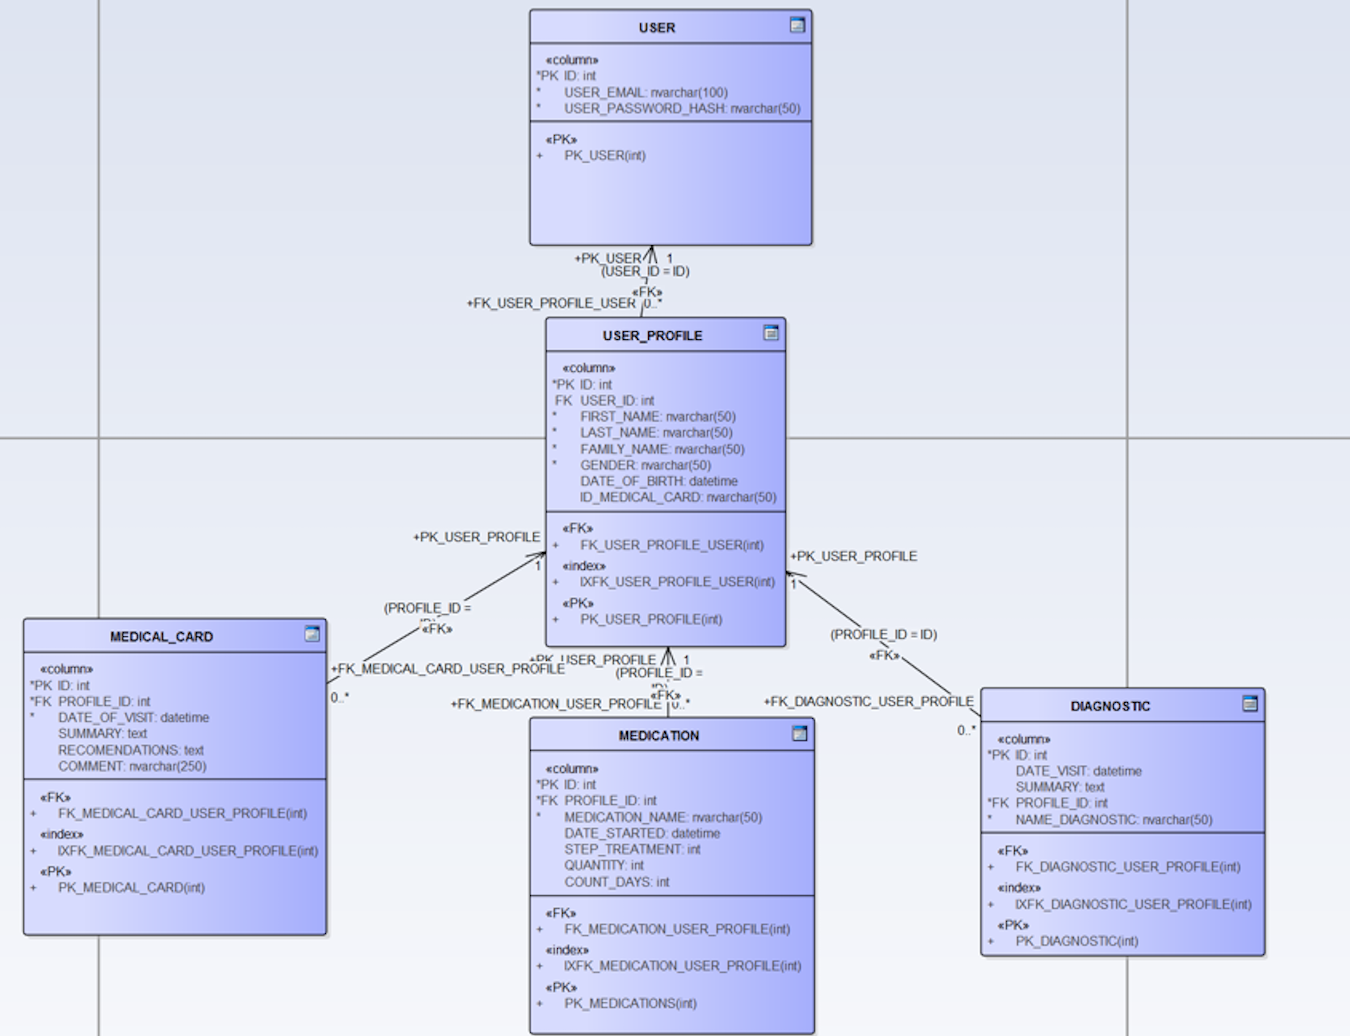
\includegraphics[scale=0.5]{db.png}  
  \caption{ Диаграмма развертывания. }
  \label{fig:domain:manual_structure:credit_db}
\end{figure}